\documentclass[11pt,a4paper]{article}
\usepackage{fontspec}
\setmainfont{TeX Gyre Pagella}
\newfontfamily\headfont{Inter}[UprightFont=*-ExtraBold,BoldFont=*-ExtraBold,Extension=.otf,Path=/usr/share/fonts/opentype/inter/]
\usepackage[a4paper,margin=2.3cm]{geometry}
\usepackage{graphicx,booktabs,float,caption,array,xcolor,longtable}
\usepackage{xurl}
\usepackage[hidelinks]{hyperref}
\usepackage{titlesec}
\usepackage[round]{natbib}
\usepackage{setspace}
\setstretch{1.05}
\renewcommand{\topfraction}{0.9}
\renewcommand{\bottomfraction}{0.8}
\renewcommand{\textfraction}{0.1}
\renewcommand{\floatpagefraction}{0.75}
\setlength{\parindent}{0pt}
\setlength{\parskip}{0.55em}
\titleformat{\section}{\headfont\Large}{\thesection}{0.8em}{}
\titleformat{\subsection}{\headfont\large}{\thesubsection}{0.8em}{}
\captionsetup{font=small,labelfont=bf}
\urlstyle{same}
\hypersetup{pdftitle={Pilgrim Roads},pdfauthor={Tristan Hotham}}

\begin{document}
\begin{center}
{\Large\bfseries Pilgrim Roads\par}
\vspace{0.4em}
{\large Mapping the waymarked pilgrimage routes and places of OpenStreetMap and Wikidata:\\77,804 km of routes and 1,330 pilgrimage sites\par}
\vspace{1.2em}
{\large Tristan Hotham\par}
\vspace{0.3em}
{\small Independent researcher\\
ORCID: 0000-0003-4931-9349\\
DOI: https://doi.org/10.5281/zenodo.23878608\par}
\vspace{0.8em}
2026
\end{center}

\begin{quote}
\small
\begin{center}\textbf{Abstract}\end{center}
I measure the waymarked pilgrimage routes recorded in OpenStreetMap and the pilgrimage sites recorded in Wikidata. From 1,906 OpenStreetMap route relations tagged as pilgrimage routes I keep 1,893, split their ways into unique segments so that no stretch of path shared by several relations is counted twice, and assign each segment to a country and to a route family. The result is 77,804 km of pilgrim routes in 34 countries, 6.3\% less than the naive sum of all relations. The Camino de Santiago accounts for 41,674 km (54\%) in 22 countries, and Germany has more of it (14,814 km) than Spain (9,922 km), followed by Poland (5,289 km). Only 13\% of the waymarked Camino lies within 500 km of Santiago; half lies more than 1,659 km away, and the farthest stretch, in Ukraine, is 2,911 km from the cathedral. The Via Francigena (5,120 km), the St Olav Ways (3,011 km) and the Marian ways of central Europe (6,750 km) make up most of the rest. Wikidata lists 1,330 pilgrimage sites in 70 countries, led by Germany, Italy, Spain and Japan, where 108 sites lie on Shikoku. Both sources are heavily European: 99.2\% of route kilometres and 73\% of sites. The largest pilgrimages in the world, to Mecca, Karbala and the Kumbh Mela, are absent from the route data, and some of the best known Christian routes are missing from the extract. The figures describe what volunteers have mapped, not where pilgrims walk.

\textbf{Keywords:} pilgrimage; Camino de Santiago; Way of St James; Via Francigena; St Olav Ways; OpenStreetMap; Wikidata; volunteered geographic information; mapping
\end{quote}

\section{Introduction}
Pilgrimage is one of the oldest reasons for long journeys on foot, and in Europe it has had a striking revival. The Camino de Santiago, which tradition traces to the early ninth century, was declared one of the three great pilgrimages of Christendom after 1492, with Jerusalem and Rome \citep{wikicamino}. In 1985 the Pilgrim's Office in Santiago issued 690 certificates of completion; in 2025 it issued 530,772. Alongside the revival, St James societies, hiking clubs and parishes have waymarked routes far beyond Spain, and the Via Francigena to Rome \citep{wikivf}, the St Olav Ways to Trondheim \citep{wikiolav} and many lesser pilgrim paths have been signed and promoted.

OpenStreetMap volunteers record such waymarked routes as route relations, and many are tagged as pilgrimage routes. Wikidata lists places of pilgrimage. Together they offer a first open, measurable picture of the world's pilgrim roads. This paper asks four questions. How many kilometres of waymarked pilgrimage route are mapped, and where? How is the Camino de Santiago, the largest network, distributed in space? Which other route families and long routes stand out? And where are the pilgrimage sites? Throughout, the emphasis is on what the open data can and cannot show. The paper accompanies an interactive map (\url{https://maps.tristanhotham.com/pilgrim-roads/}).

\section{Data}
\textbf{Routes.} An extract of OpenStreetMap \citep{osm} downloaded through the Overpass API in 2026: route relations tagged as pilgrimage routes, or linked to Wikidata pilgrim route items. Of 2,028 relation ids requested, 5 batches (100 ids, 4.9\%) failed and are missing; 1,906 relations were returned with their tags, the geometry of their ways (coordinates to four decimal places) and the ids of child relations. 1,704 carry a pilgrimage tag and 368 a Wikidata link.

\textbf{Pilgrim route items.} A Wikidata \citep{wikidata} query (run with QLever) for items that are pilgrim routes or parts of the Way of St James: 1,862 items, of which 1,458 are stations of the cross and 404 are routes. These are used to classify relations and to check the extract's coverage.

\textbf{Sites.} A Wikidata query for pilgrimage sites, with coordinates, country and religion: 1,403 rows, 1,330 distinct items, 160 without an English label.

\textbf{Context.} English Wikipedia articles on the Way of St James, the Via Francigena, the Shikoku pilgrimage, St Olav's Way, the Kumano Kodō, the Hajj, the Arba'een pilgrimage and the Kumbh Mela \citep{wikicamino,wikivf,wikishikoku,wikiolav,wikikumano,wikihajj,wikiarbaeen,wikikumbh} supply historical facts, route lengths and the yearly certificate counts. Country outlines and populations come from Natural Earth \citep{naturalearth}.

\section{Methods}
\subsection{Selecting relations}
I keep every relation except those whose route tag is a road, bus route, ski piste or fitness trail, three network relations, and six that inspection showed are not pilgrimage routes (a forest trail named after the Pilgrim River in Michigan, a recreational rail trail in Texas, two ecological trails in Colombia, a park walk in Canberra and a running route in York). That leaves 1,893 relations: 1,769 without child relations and 124 containers (63 of them super-routes). Containers list 1,039 child relations, 280 of which are not in the extract; 17 containers have none of their children.

\subsection{Counting each stretch once}
The same path often belongs to several relations: a stage and the super-route it belongs to, two routes that share a valley, a walking and a cycling version, or a way listed twice. I split every way into consecutive point pairs, treat a pair as the same segment whichever direction it is drawn in, and keep each segment once. The 341,659 ways with 1,060,346 points give 671,288 segments, of which 626,144 are unique. The great circle length of the raw segments is 83,037 km; of the unique segments, 77,804 km. Because the coordinates are rounded to about 10 m, two separately drawn but parallel paths are not merged; I found no sign that this matters at the scale reported. Each segment is placed in the Natural Earth 1:10m country containing its midpoint; 77 km fall just outside every outline, on coasts and estuaries.

\subsection{Route families}
Each relation is assigned to one family. A relation is Camino de Santiago if any of its names (in any language), its pilgrimage, symbol or Wikipedia tags mention St James or Santiago (Jakobsweg, Droga św. Jakuba, Svatojakubská cesta, Camí de Sant Jaume and so on), if it links to the Wikidata item for the Way of St James, or if its symbol is a scallop shell; Via Francigena, St Olav Ways and Marian ways are recognised by similar rules (common.py in the code lists them). A relation with no telling name inherits the family of its nearest classified parent, and a container still unplaced takes the family of most of its children's length. Table~\ref{tab:fams} shows how each family's relations were placed. A family's kilometres include every segment any of its relations uses; 1,591 km are used by more than one family and so count in each.

\subsection{Distance from Santiago and route length}
For the Camino I measure the great circle distance from the cathedral of Santiago de Compostela (42.8806°N, 8.5446°W) to each segment's midpoint. This is distance as the crow flies, not walking distance. Route length is reported in two ways: for a top-level relation (one that is not the child of another) with all its descendants, segments counted once; and for single relations with no children, on their own ways.

\subsection{Sites}
Each site's country is the one Wikidata gives, checked against its coordinates (where Wikidata gives more than one country, the one containing the point). Tradition comes from Wikidata's religion values where present, grouped as Christian, Buddhist, Muslim and so on. For a second, rougher reading I also assign a tradition from the site's name (``church'', ``Wallfahrtskirche'', ``Santuário'', ``-ji temple'', ``mausoleum'') where no religion is recorded. Rates per million people use Natural Earth population estimates. To ask whether the mapped routes lead to the listed sites, I measure each site's distance to the nearest point of any route.

\begin{table}[tbp]\centering\footnotesize\setlength{\tabcolsep}{4pt}\caption{Route families: relations, unique kilometres, share of all route kilometres, countries, the leading country, and how the relations were placed (by name or Wikidata link, by scallop shell symbol, or from a parent or children).}\label{tab:fams}\begin{tabular}{lrrrrlrrr}\toprule Family & Relations & km & Share & Countries & Leading country & Name/WD & Shell & Inherited\\\midrule
Camino de Santiago & 728 & 41,674 & 53.6\% & 22 & Germany (36\%) & 646 & 78 & 4\\
Via Francigena & 119 & 5,120 & 6.6\% & 5 & Italy (74\%) & 119 & 0 & 0\\
St Olav Ways & 53 & 3,011 & 3.9\% & 3 & Norway (68\%) & 53 & 0 & 0\\
Marian ways & 271 & 6,750 & 8.7\% & 11 & Hungary (36\%) & 270 & 0 & 1\\
Other pilgrim routes & 722 & 22,862 & 29.4\% & 26 & Germany (30\%) & 0 & 0 & 127\\
\midrule All routes & 1,893 & 77,804 & & 34 & Germany (28\%) & & & \\
\bottomrule\end{tabular}\end{table}

\section{Results}
\subsection{How much and where}
The extract holds 77,804 km of unique waymarked pilgrim route in 34 countries (Figure~\ref{fig:map}). Germany has the most (21,446 km, 28\%), then Spain (10,367 km), Italy (10,127 km), Poland (5,616 km), Hungary (4,678 km) and Austria (4,626 km). Only 564 km lie outside Europe, in 5 countries: Brazil (368 km, one route to the shrine of Aparecida), Japan (141 km, mostly the Kumano Kodō, \citealp{wikikumano}) and short paths in Israel, India and elsewhere in Asia.

\begin{figure}[tbp]\centering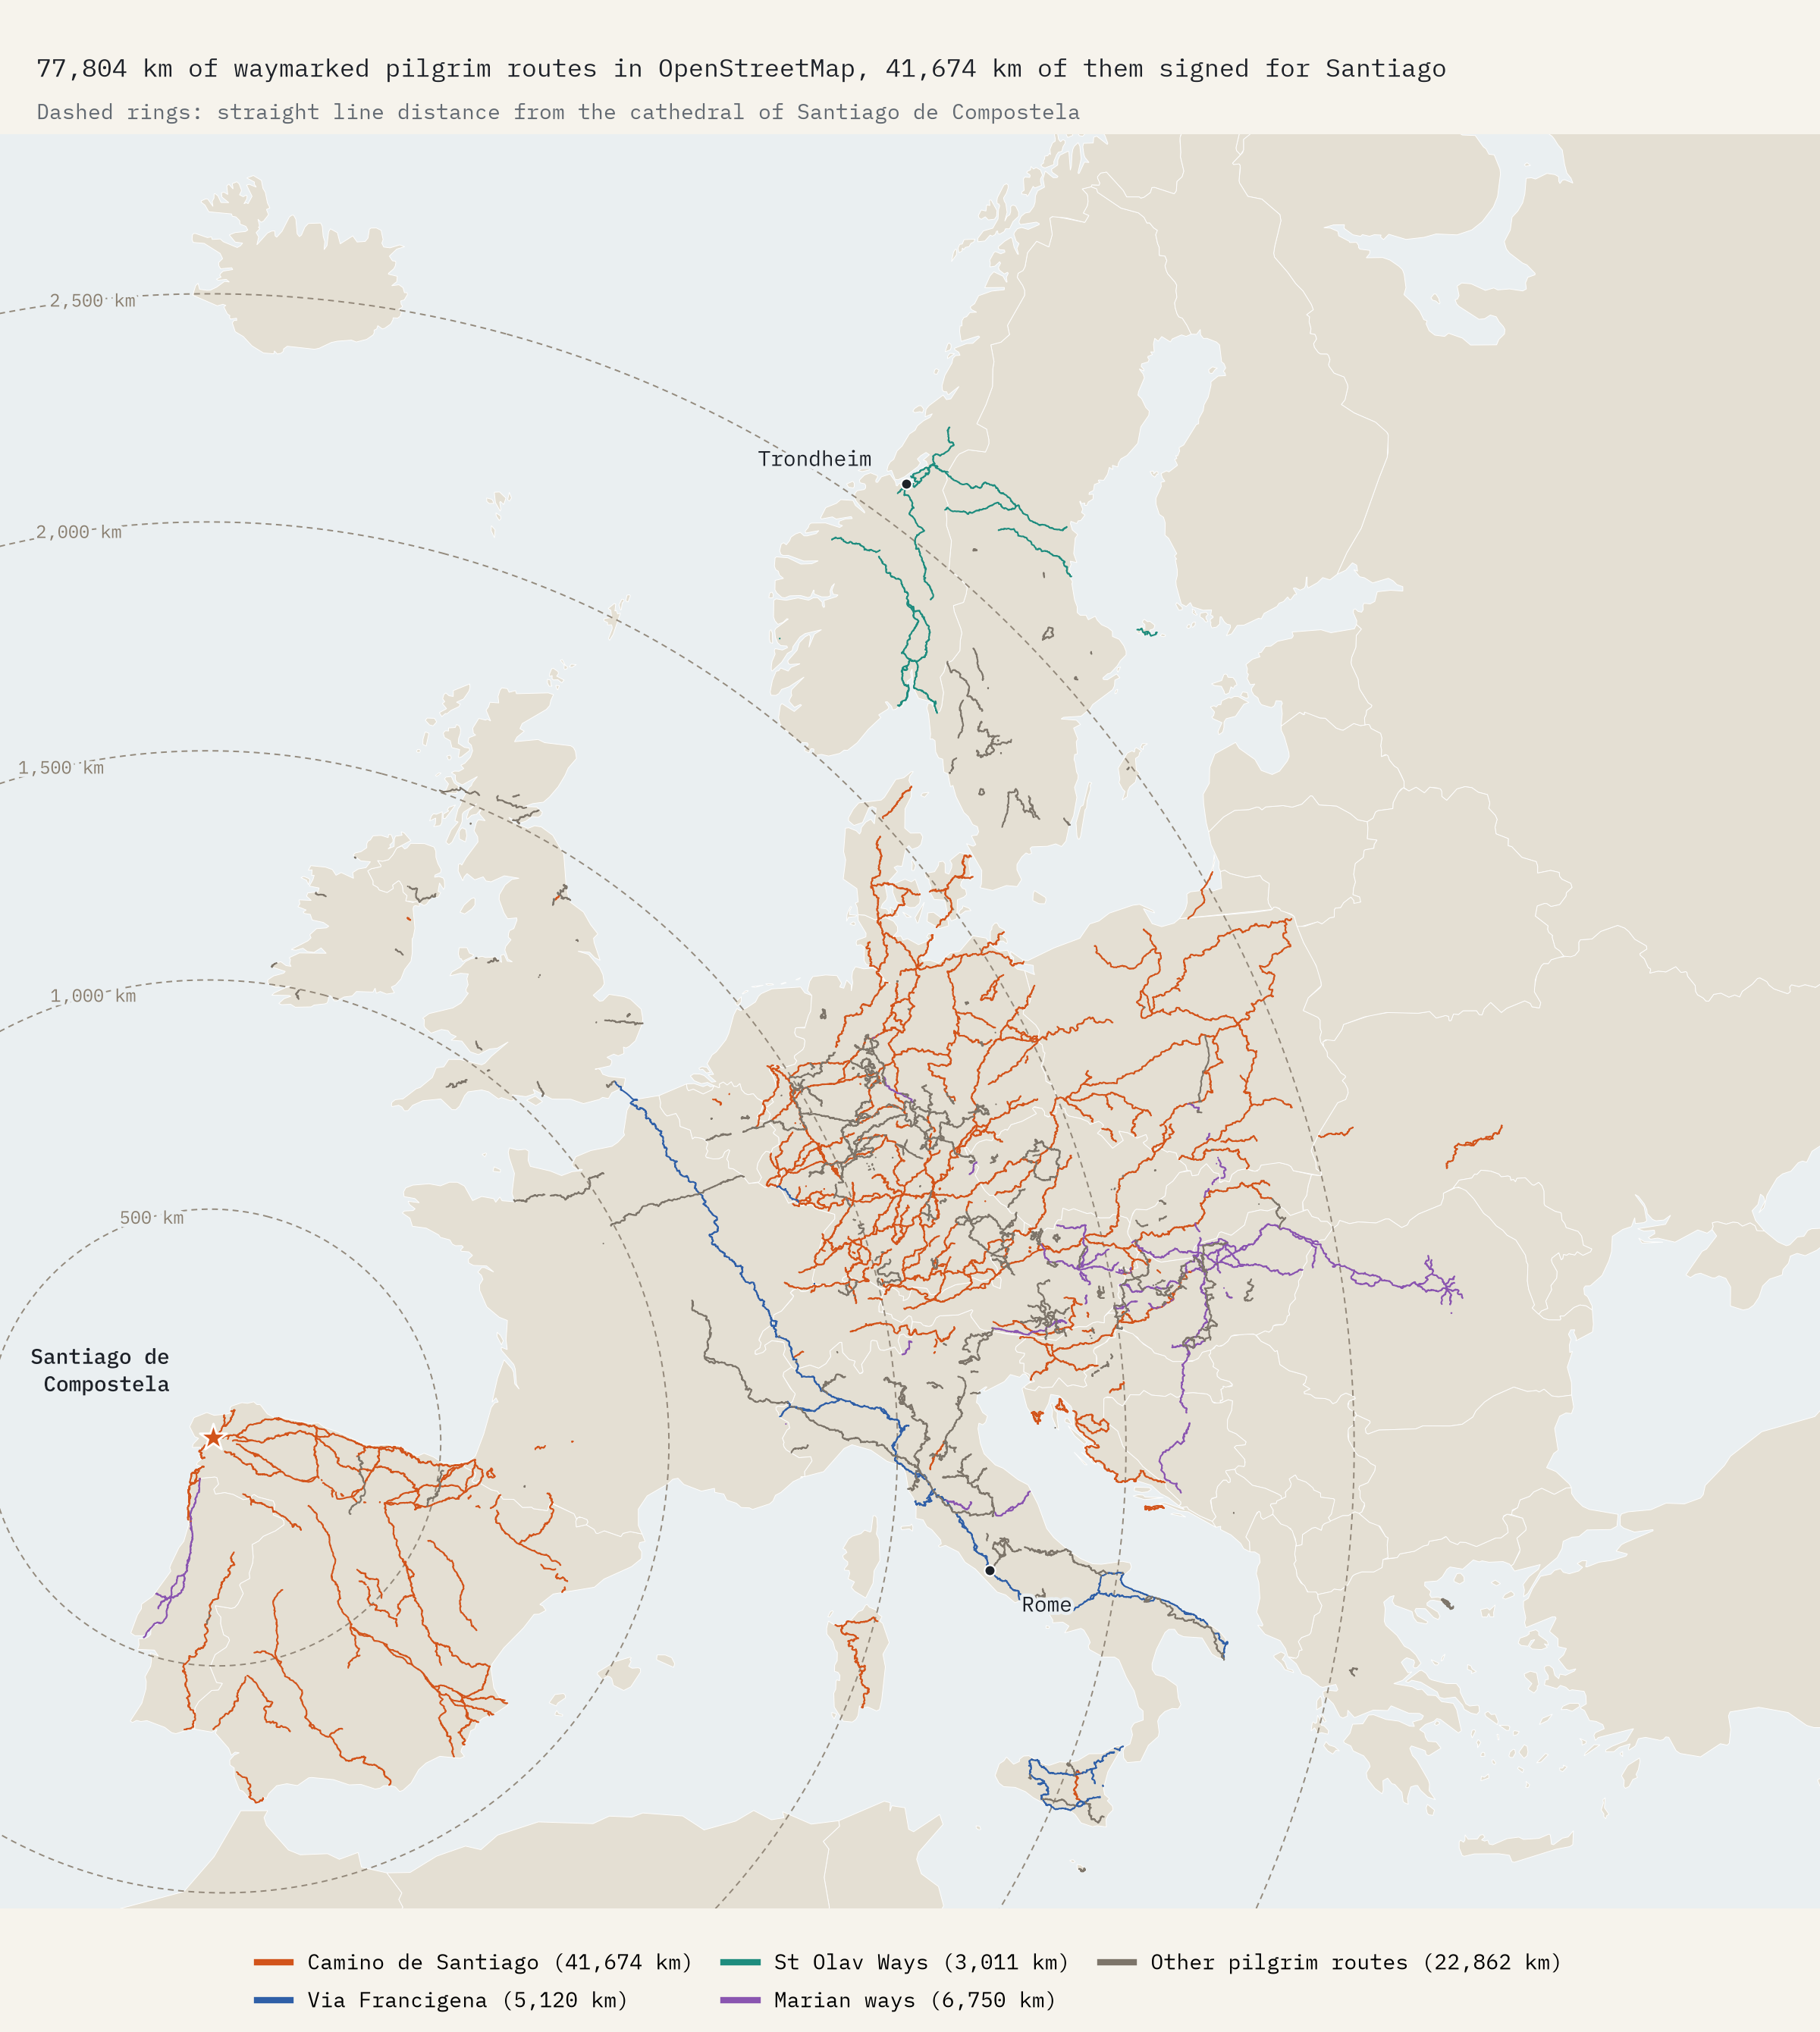
\includegraphics[width=.92\textwidth]{f_map.png}
\caption{Waymarked pilgrim routes in Europe by family, with rings at 500 km intervals from the cathedral of Santiago de Compostela. Lines simplified for display.}\label{fig:map}\end{figure}

\subsection{The Camino de Santiago}
The Camino accounts for 41,674 km (54\% of the total) in 22 countries (Figure~\ref{fig:camino}, Table~\ref{tab:camino}). Germany has 14,814 km (36\%), 1.49 times Spain's 9,922 km (24\%); Poland has 5,289 km. Outside Spain and Portugal lie 74\% of the network. France, with 462 km, is clearly under-represented: several of its historic routes are among the relations missing from the extract (Section~\ref{sec:cov}), and others are probably mapped as long distance hiking trails without pilgrimage tags. The Spanish figure is also an undercount, since several stages of the Camino Francés, including its final stretch into Santiago, are missing.

\begin{figure}[tbp]\centering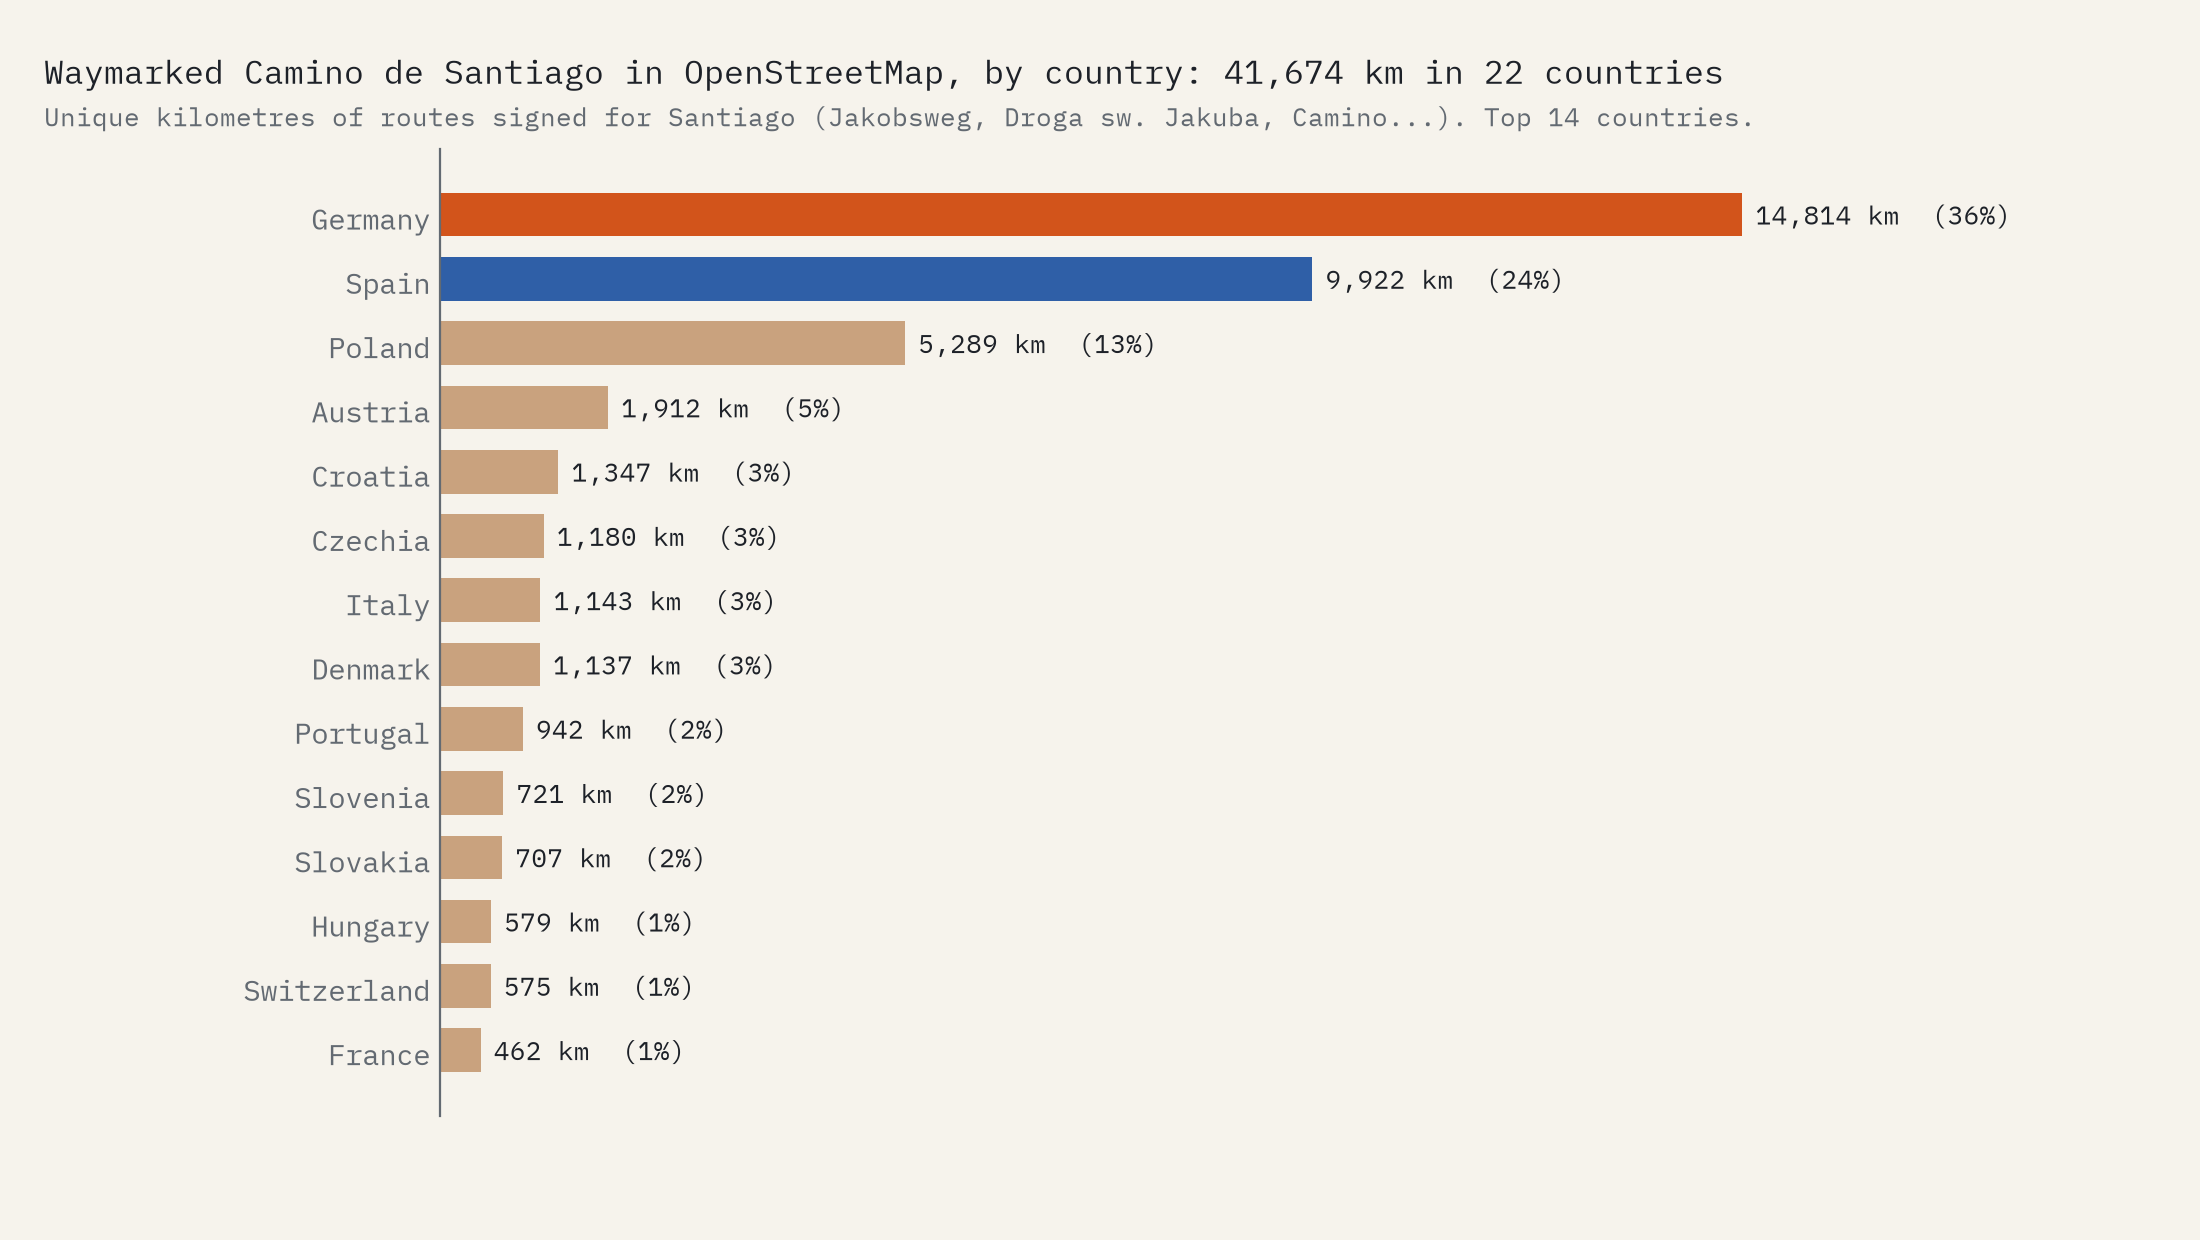
\includegraphics[width=\textwidth]{f_camino.png}
\caption{Unique kilometres of waymarked Camino de Santiago in OpenStreetMap, by country (top 14).}\label{fig:camino}\end{figure}

\begin{table}[tbp]\centering\small\caption{Waymarked Camino de Santiago by country (top 15): unique kilometres and share of the Camino total.}\label{tab:camino}\begin{tabular}{lrr}\toprule Country & km & Share\\\midrule
Germany & 14,814 & 35.5\%\\
Spain & 9,922 & 23.8\%\\
Poland & 5,289 & 12.7\%\\
Austria & 1,912 & 4.6\%\\
Croatia & 1,347 & 3.2\%\\
Czechia & 1,180 & 2.8\%\\
Italy & 1,143 & 2.7\%\\
Denmark & 1,137 & 2.7\%\\
Portugal & 942 & 2.3\%\\
Slovenia & 721 & 1.7\%\\
Slovakia & 707 & 1.7\%\\
Hungary & 579 & 1.4\%\\
Switzerland & 575 & 1.4\%\\
France & 462 & 1.1\%\\
Ukraine & 440 & 1.1\%\\
\midrule All 22 countries & 41,674 & 100\%\\
\bottomrule\end{tabular}\end{table}

Measured from the cathedral, the network is strikingly remote from its goal (Figure~\ref{fig:bands}). Only 13\% lies within 500 km (777 km within 100 km); half lies more than 1,659 km away; and 74\% more than 1,000 km away. The band from 1,500 to 2,000 km holds 41\%, mostly in Germany, Austria and Croatia, and the band beyond 2,000 km, mostly in Poland, another 19\%. The farthest stretch is the Camino Podolico at Vinnytsya in Ukraine, 2,911 km from Santiago; the northernmost reaches 57.4°N in Denmark.

\begin{figure}[tbp]\centering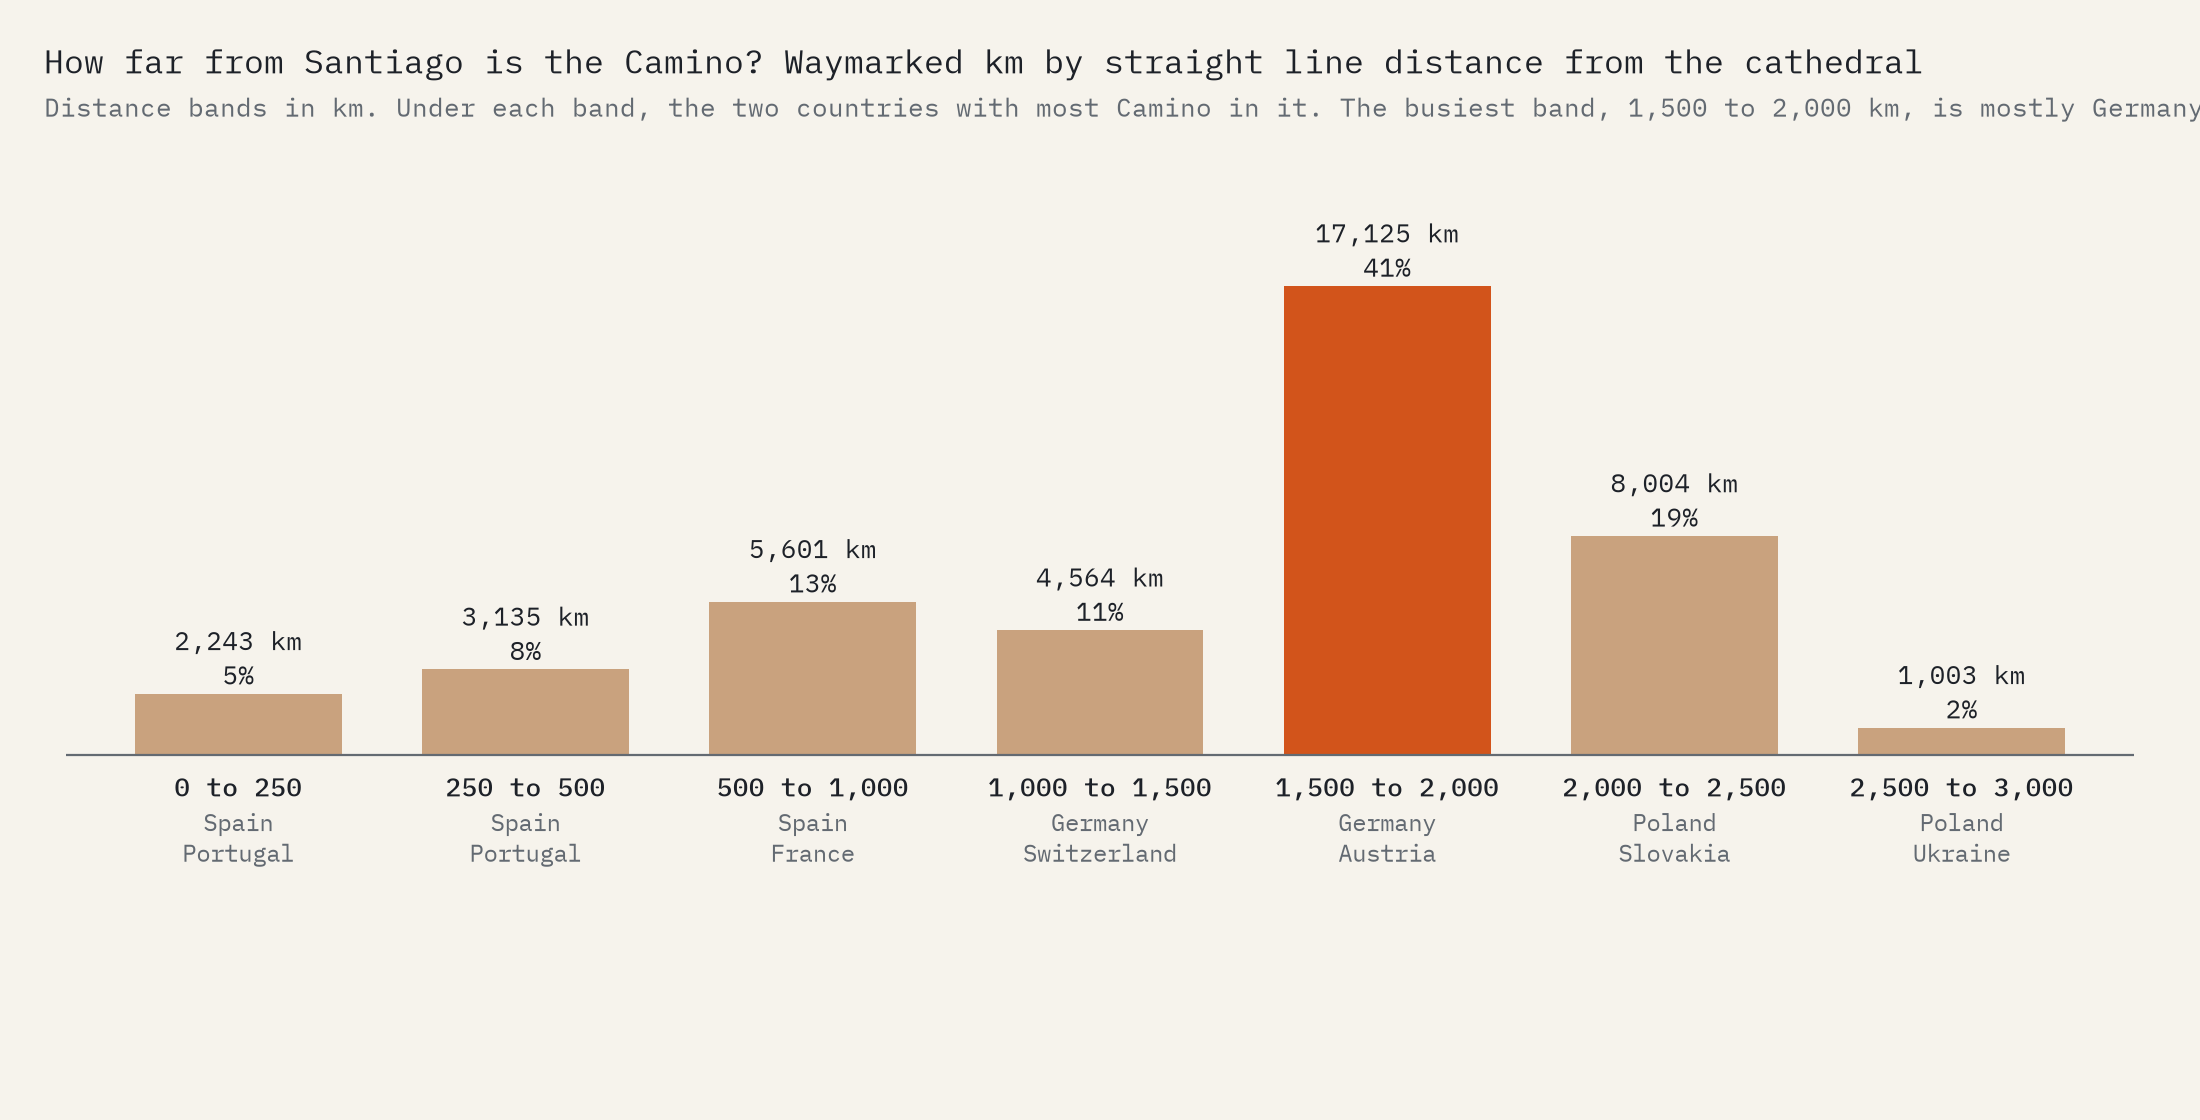
\includegraphics[width=\textwidth]{f_bands.png}
\caption{Waymarked Camino kilometres by great circle distance from the cathedral of Santiago de Compostela.}\label{fig:bands}\end{figure}

\subsection{Other families and the longest routes}
The Via Francigena has 5,120 km, 74\% of it in Italy; Sigeric's itinerary of around 990 had 80 stages and some 1,700 km \citep{wikivf}, but the mapped system also includes variants, the extension south of Rome and the Francigene of Sicily. The St Olav Ways have 3,011 km, 68\% in Norway and most of the rest in Sweden, against about 640 km for the main route from Oslo \citep{wikiolav}. The Marian ways have 6,750 km, 36\% in Hungary, most of them the Via Mariae network, with Portugal's routes to Fátima adding 743 km. Other routes, from the Lutherweg to the roads to Assisi, total 22,862 km.

Among 1,129 top-level route systems, the longest is the Via Francigena at 3,944 km, followed by the regional Jakobsweg networks of Bavaria (2,696 km) and Baden-Württemberg (2,227 km) (Figure~\ref{fig:longest}, Table~\ref{tab:longest}). Among single relations without children the longest is the Camino de Santiago del Sureste (923 km), then the Wanderroute Via Nova (852 km); the median single relation is 21.1 km long, because most routes are mapped stage by stage.

\begin{figure}[tbp]\centering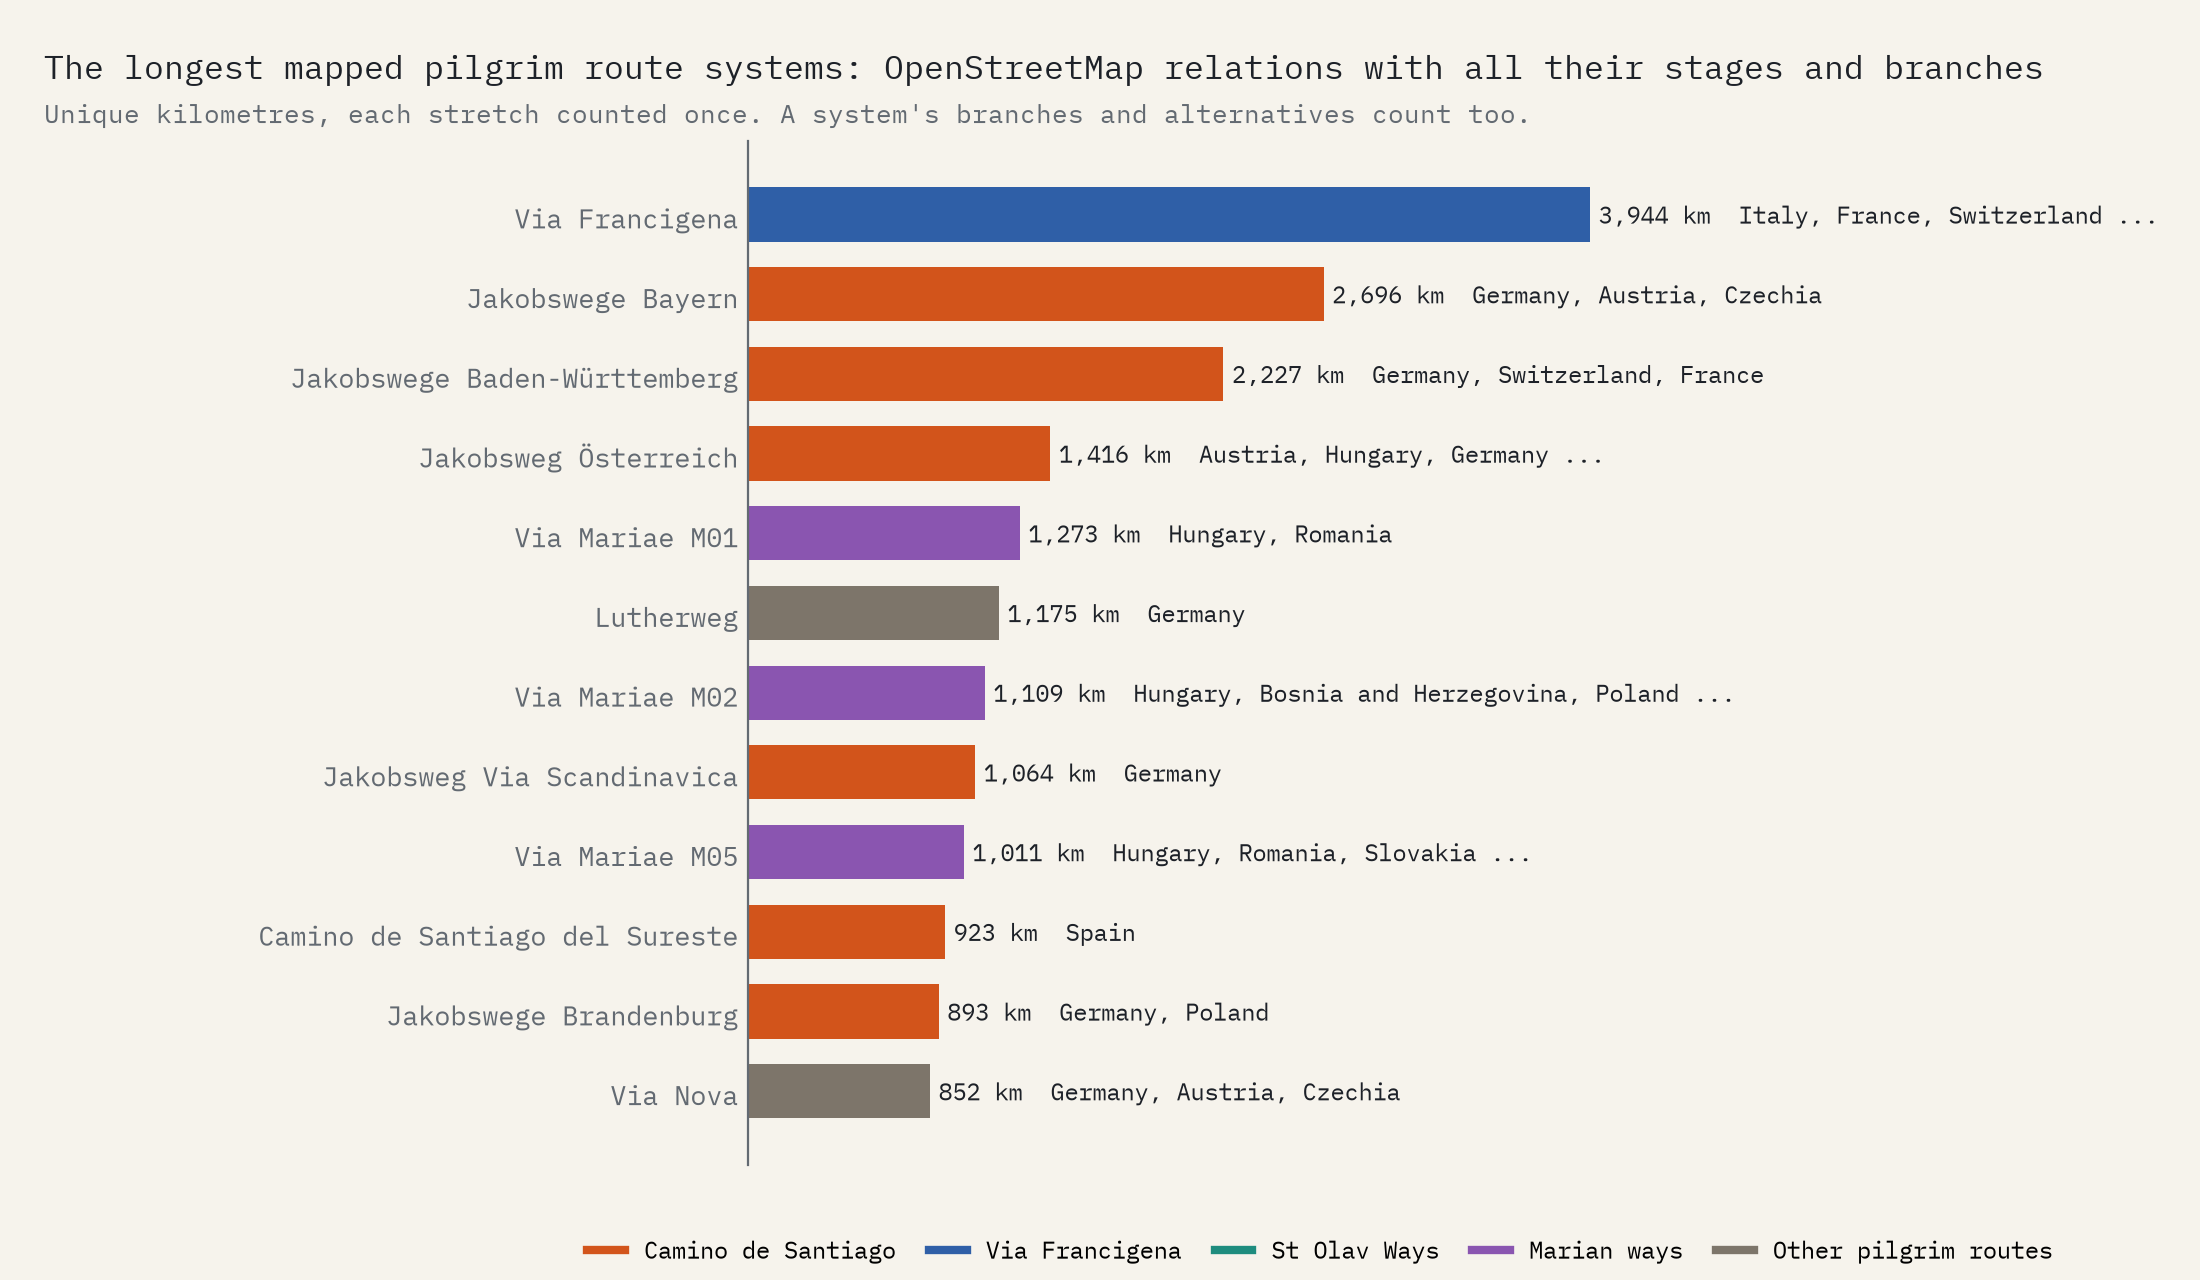
\includegraphics[width=\textwidth]{f_longest.png}
\caption{The longest top-level pilgrim route systems, with all their stages and branches, coloured by family.}\label{fig:longest}\end{figure}

\begin{table}[tbp]\centering\footnotesize\setlength{\tabcolsep}{4pt}\caption{The fifteen longest top-level route systems: unique kilometres with all descendants, the length in the relation's distance tag where given, and countries in order of length.}\label{tab:longest}\begin{tabular}{p{4.6cm}p{2.6cm}rrp{4.4cm}}\toprule System & Family & km & Tag & Countries\\\midrule
Via Francigena & Via Francigena & 3,944 & 3268 & Italy, France, Switzerland, United Kingdom\\
Jakobswege Bayern & Camino de Santiago & 2,696 &  & Germany, Austria, Czechia\\
Jakobswege Baden-Württemberg & Camino de Santiago & 2,227 &  & Germany, Switzerland, France\\
Jakobsweg Österreich & Camino de Santiago & 1,416 &  & Austria, Hungary, Germany, Slovenia and others\\
Via Mariae M01 & Marian ways & 1,273 & 1330 & Hungary, Romania\\
Lutherweg & Other pilgrim routes & 1,175 &  & Germany\\
Via Mariae M02 & Marian ways & 1,109 &  & Hungary, Bosnia and Herzegovina, Poland, Slovakia and others\\
Jakobsweg Via Scandinavica & Camino de Santiago & 1,064 &  & Germany\\
Via Mariae M05 - The Central-European Pilgrimw & Marian ways & 1,011 &  & Hungary, Romania, Slovakia, Austria\\
Camino de Santiago del Sureste & Camino de Santiago & 923 &  & Spain\\
Jakobswege Brandenburg & Camino de Santiago & 893 &  & Germany, Poland\\
Wanderroute Via Nova & Other pilgrim routes & 852 &  & Germany, Austria, Czechia\\
Jakobova pot Slovenija & Camino de Santiago & 747 &  & Slovenia, Italy, Hungary\\
Jakobsweg via Baltica & Camino de Santiago & 722 &  & Germany, Poland\\
St. Olavsleden & St Olav Ways & 658 & 564 & Sweden, Norway\\
\bottomrule\end{tabular}\end{table}

\subsection{Pilgrimage sites}
Wikidata's 1,330 pilgrimage sites are spread over 70 countries, but Germany (239), Italy (225) and Spain (163) hold 47\% of them (Figures~\ref{fig:sites} and~\ref{fig:sitescountry}). Japan has 114, of which 108 are on Shikoku, the island of the 88 temple pilgrimage \citep{wikishikoku}; the Philippines has 51. Among countries with ten or more sites, Austria has the most per head (5.4 per million people), then Portugal (4.2) and Czechia (3.8). A religion is recorded for 677 sites (51\%), 94\% of them Christian. Adding a reading from names gives 1,023 Christian, 115 Buddhist, 8 Muslim and 7 Hindu sites, with 175 unknown. Only 332 sites (25\%; 34\% in Europe) lie within 5 km of a mapped route.

\begin{figure}[tbp]\centering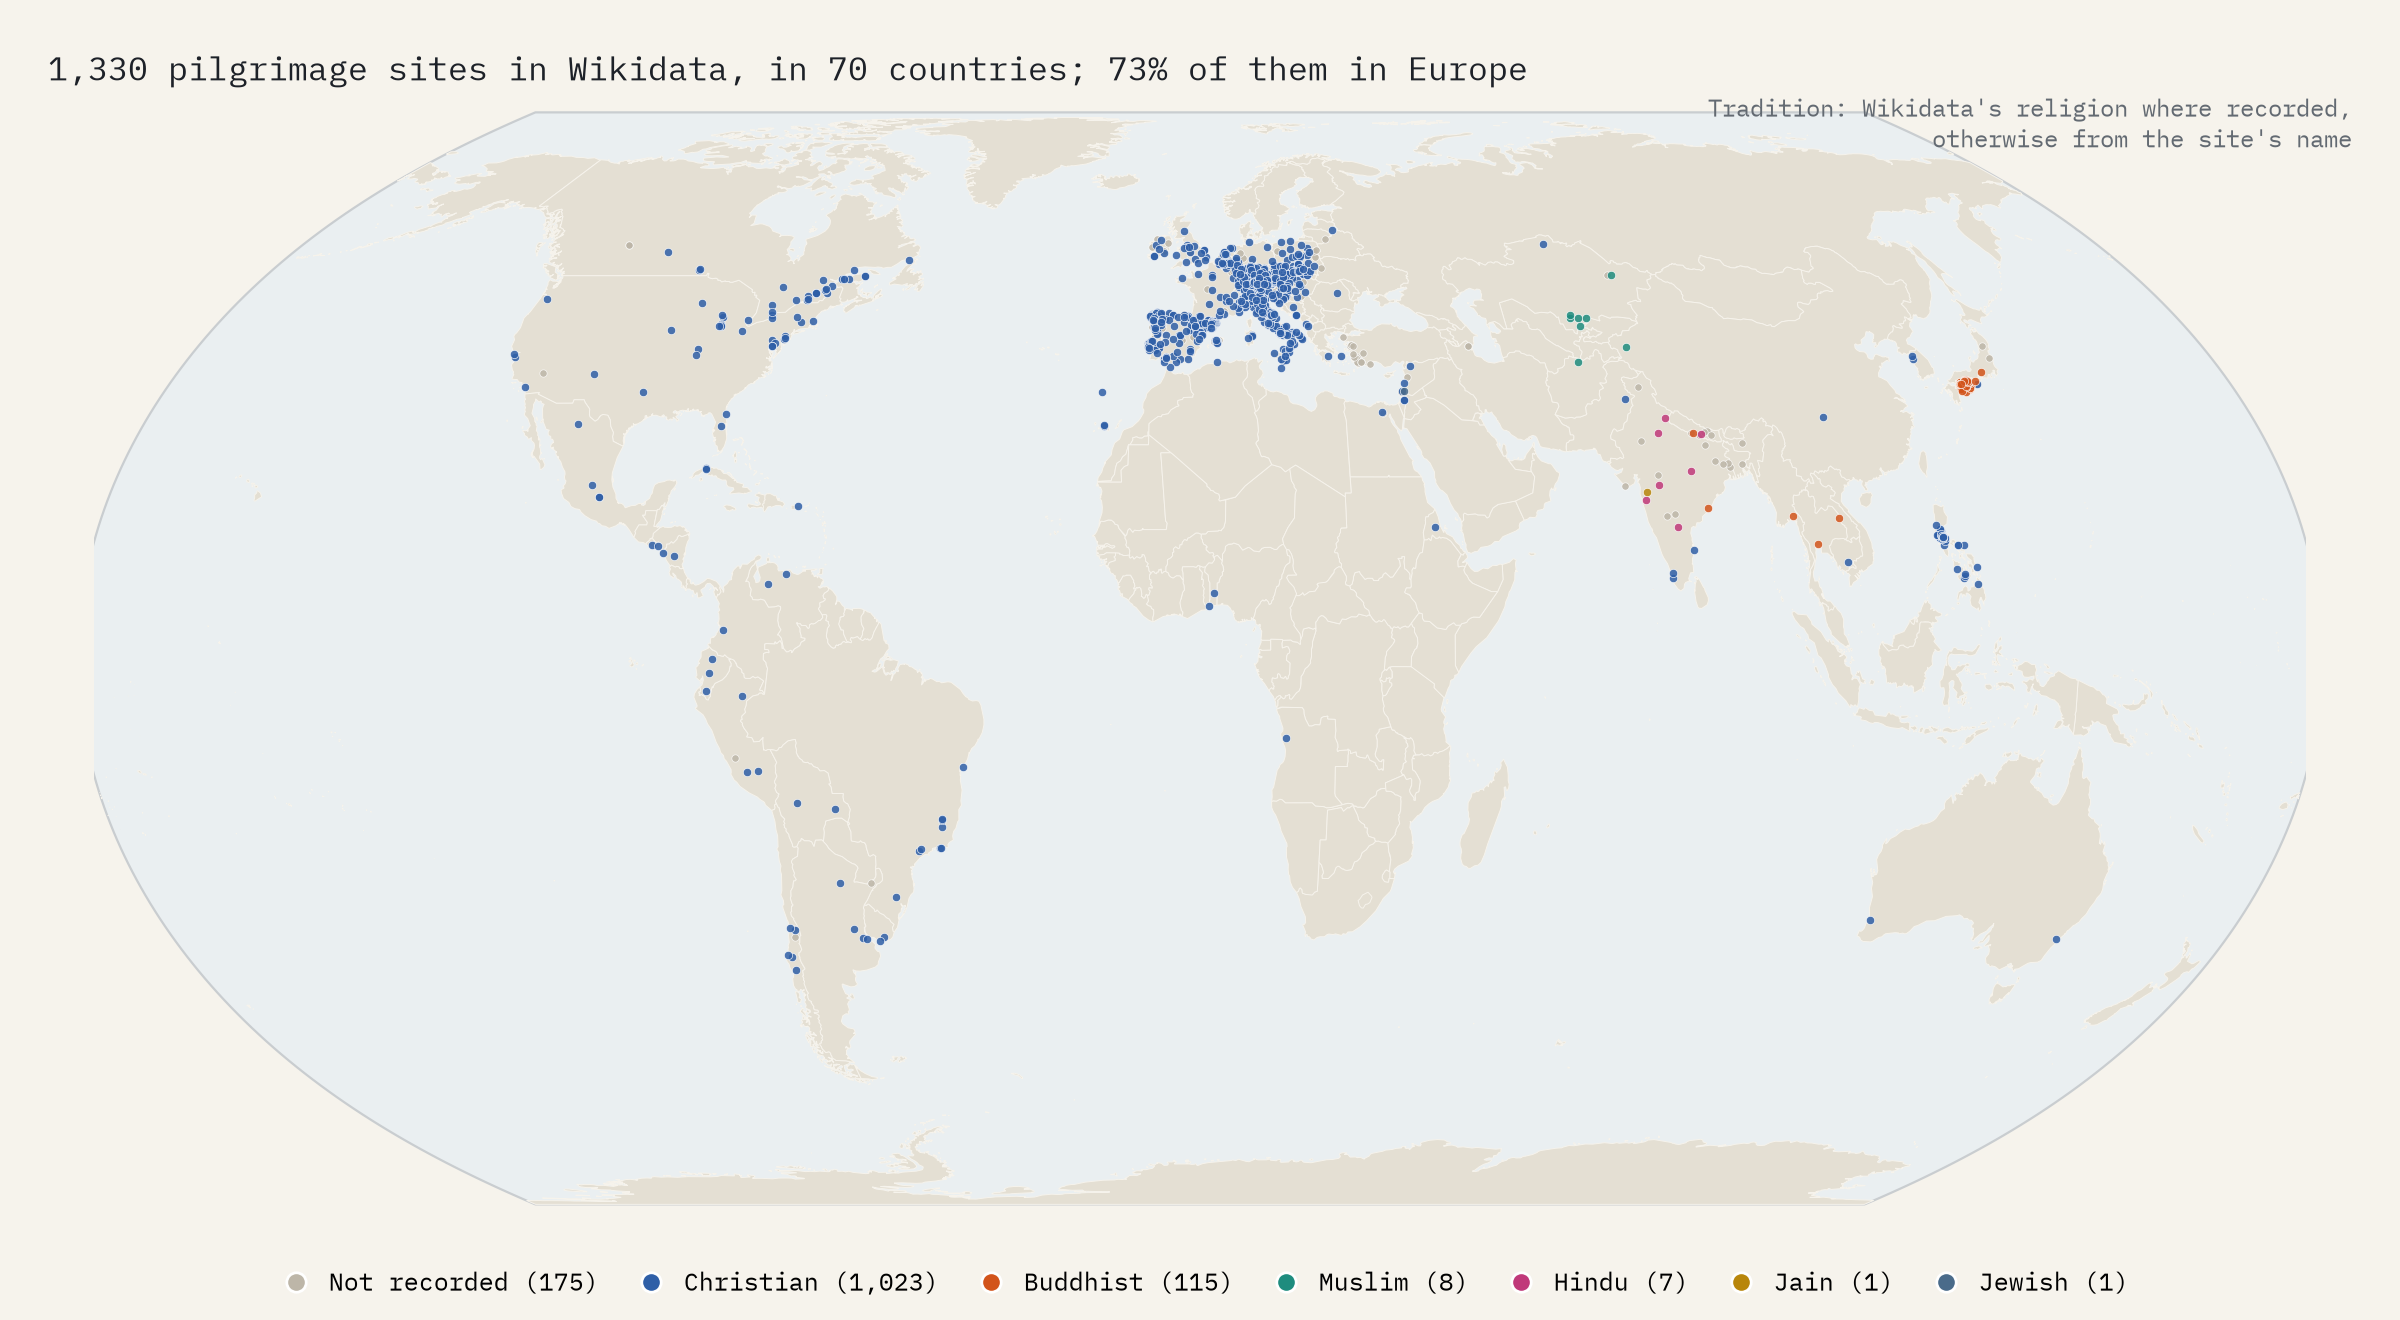
\includegraphics[width=\textwidth]{f_sites.png}
\caption{Wikidata pilgrimage sites, coloured by tradition (recorded, or read from the name).}\label{fig:sites}\end{figure}

\begin{figure}[tbp]\centering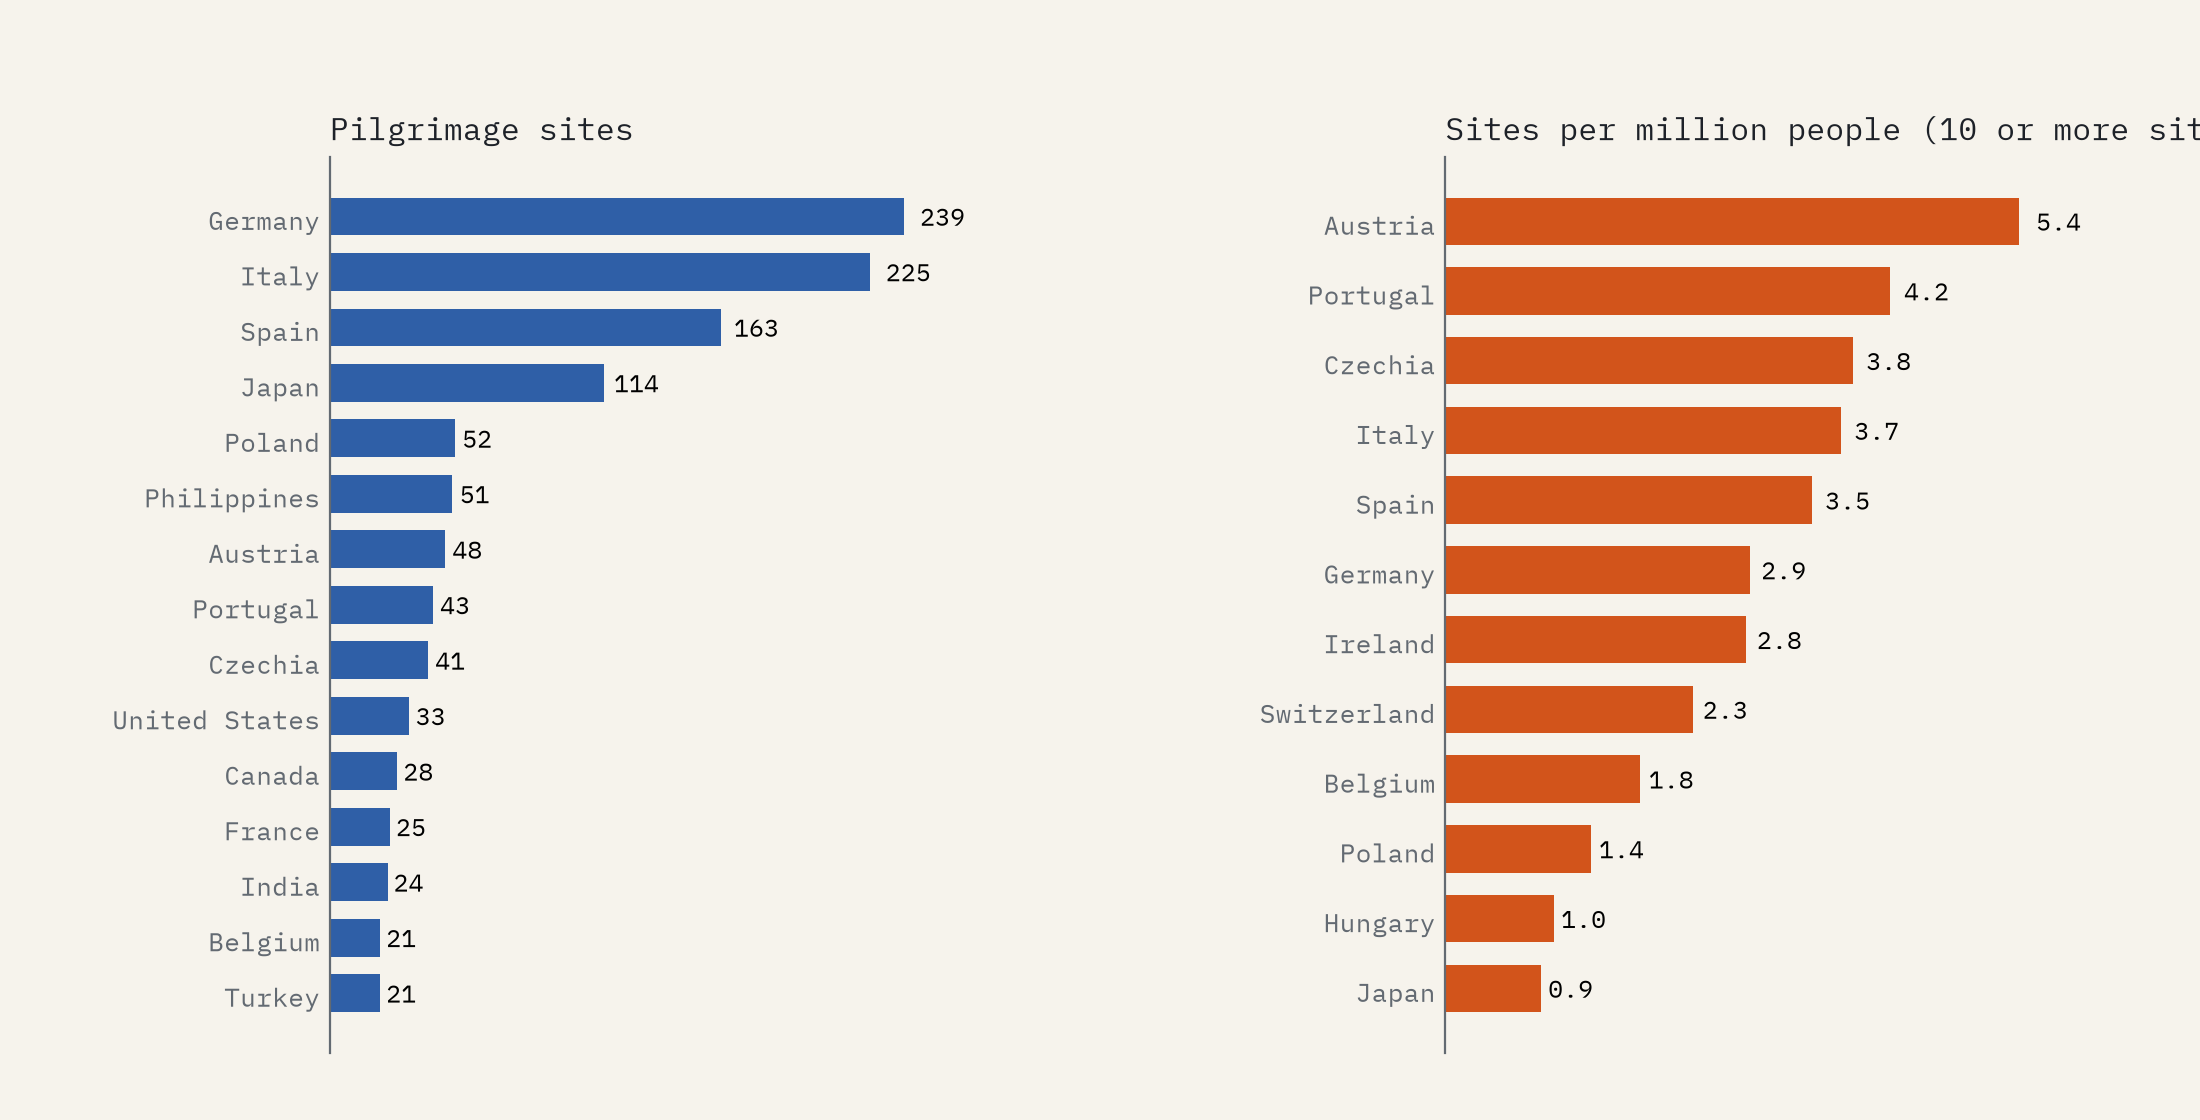
\includegraphics[width=\textwidth]{f_sites_country.png}
\caption{Pilgrimage sites by country: count (left) and per million people for countries with ten or more sites (right).}\label{fig:sitescountry}\end{figure}

\subsection{Pilgrims on the Camino}
The certificate counts (Figure~\ref{fig:comp}) rose from 690 in 1985 to 347,578 in 2019, fell to 54,144 in 2020 and reached 530,772 in 2025, 769 times the 1985 figure. Holy Years, when 25 July falls on a Sunday, stand out (1993: 99,436; 2010: 272,703). In 2024, 47\% of certificate holders walked the Camino Francés and 32\% started at Sarria \citep{wikicamino}: the pilgrims are concentrated on a small part of the network mapped here.

\begin{figure}[tbp]\centering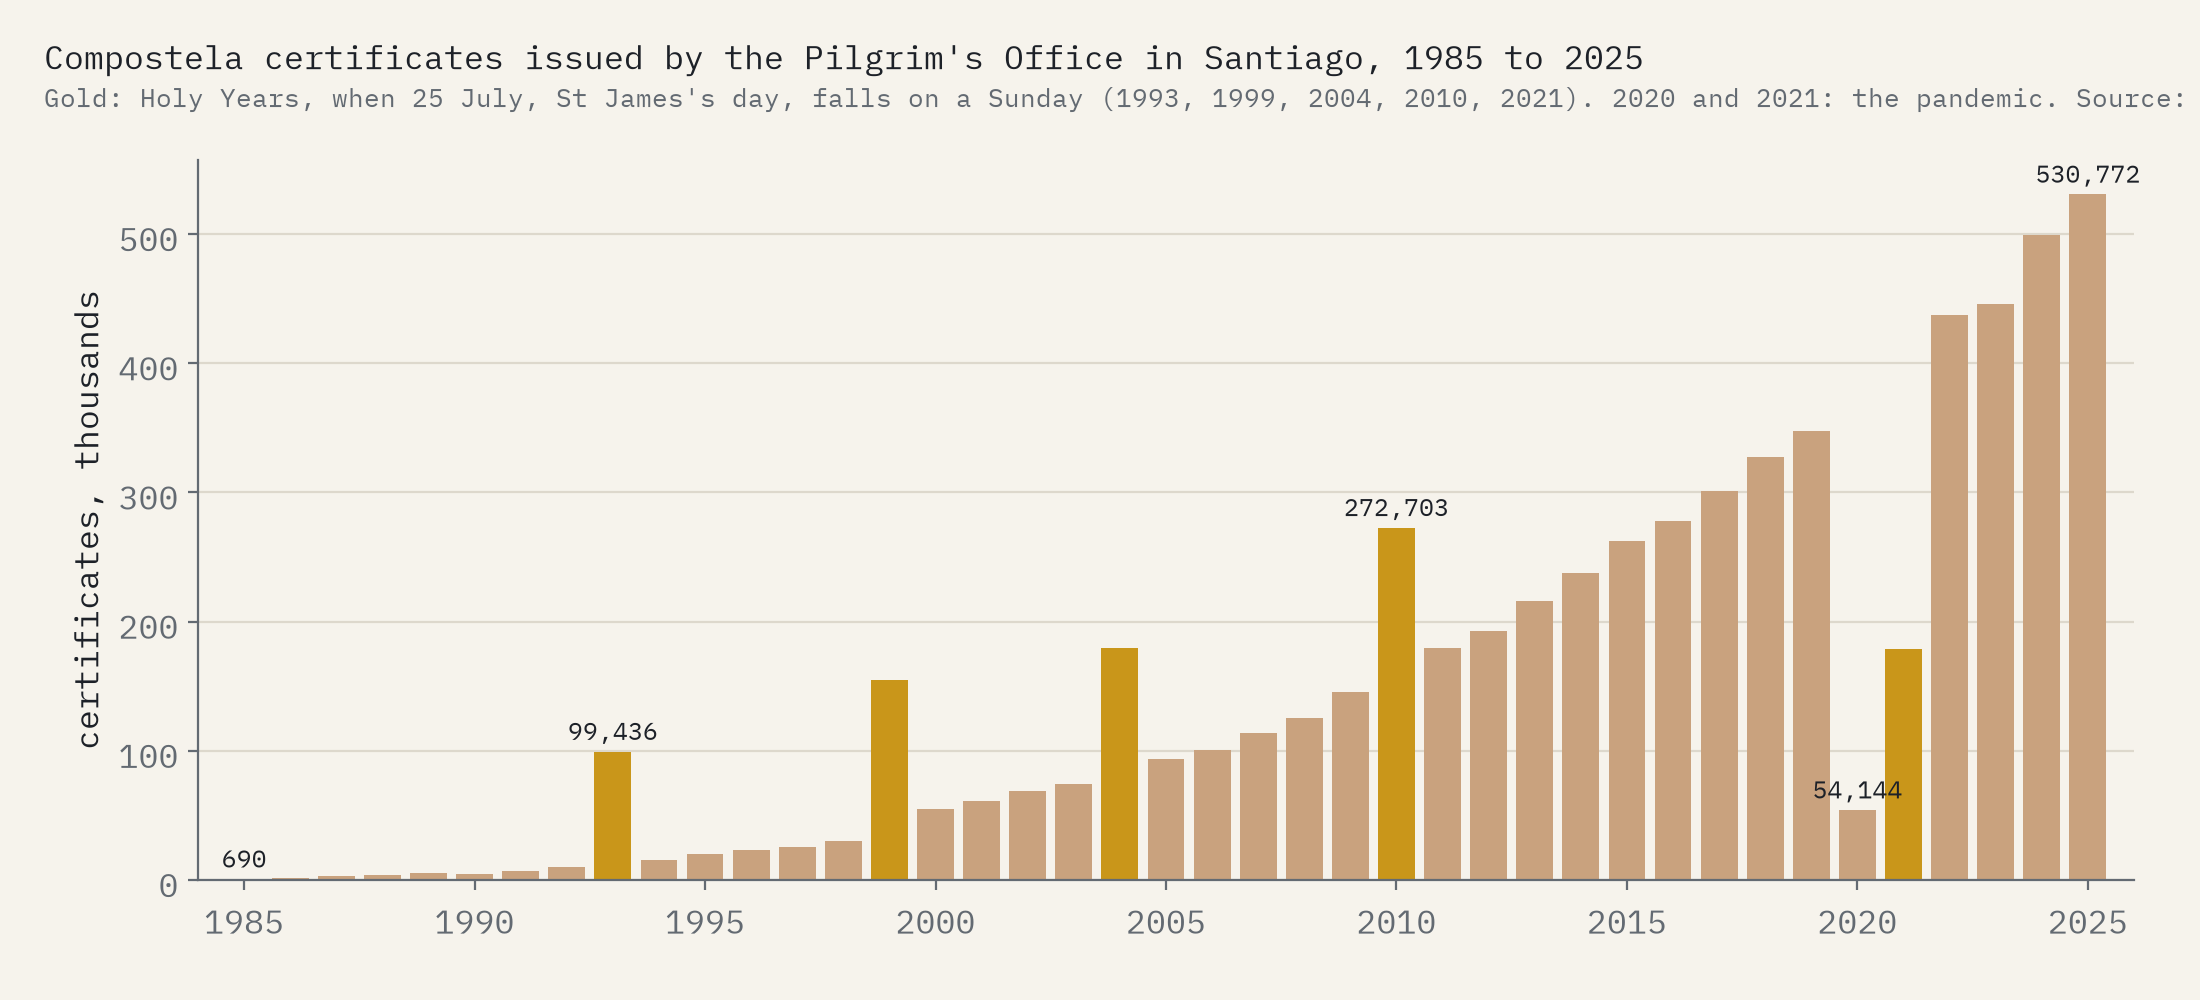
\includegraphics[width=\textwidth]{f_compostela.png}
\caption{Compostela certificates issued per year, 1985 to 2025, as tabulated in Wikipedia from the archives of Santiago de Compostela. Gold: Holy Years.}\label{fig:comp}\end{figure}

\section{Coverage and limitations}\label{sec:cov}
First, the extract is incomplete. 100 relation ids failed to download, 280 child relations listed by containers are absent, and of 41 Wikidata pilgrim route items (other than stations of the cross) that name an OpenStreetMap relation, 25 are missing, among them the Camino Francés super-route, the Via Turonensis, the Via Tolosana, the Sanabrés and Catalan ways and the Romboleden. All totals are therefore lower bounds.

Second, OpenStreetMap is volunteered: what is mapped, and how it is tagged, varies by country and community. Germany's lead over Spain on the Camino may partly reflect differences in how thoroughly each country's routes have been mapped and tagged; France's near absence reflects tagging and the missing relations, not a lack of routes.

Third, both sources are European. 99.2\% of the route kilometres and 73\% of the sites are in Europe. The largest pilgrimages are not walking routes in this sense and do not appear: the Hajj drew 1,707,301 pilgrims in 2026 \citep{wikihajj}, the Arba'een walk to Karbala draws ten to twenty million a year \citep{wikiarbaeen}, and about 660 million attended the Kumbh Mela in 2025 \citep{wikikumbh}. Historic roads such as the Darb Zubayda from Kufa to Mecca (1,300 km in Wikidata) are not mapped as routes, and the Shikoku circuit appears only through its temples.

Fourth, the family rules are keyword based and will misplace a few relations; the scallop shell rule alone placed 78 relations in the Camino. Fifth, the tradition read from site names is a rough guide. Sixth, distances from Santiago are straight lines.

\section{Conclusion}
OpenStreetMap records 77,804 km of waymarked pilgrim routes, and more than half of them lead, eventually, to Santiago. The modern Camino is not a Spanish road but a continental web whose centre of mass lies in Germany and central Europe, 1,659 km from the tomb it leads to, while the pilgrims themselves crowd onto its last few hundred kilometres. The open data show this European revival in detail, and they show almost nothing of the much larger pilgrimages of Islam and Hinduism. A map of the world's pilgrim roads made from volunteered data is, for now, a map of where those volunteers live and walk.

\section*{Data and code availability}
The interactive map is at \url{https://maps.tristanhotham.com/pilgrim-roads/}. Data and code are at \url{https://github.com/Tristan-Hotham/pilgrim-roads} and archived with this paper at https://doi.org/10.5281/zenodo.23878608. Text, figures and derived data are released under CC BY 4.0, except the route geometry and route table derived from OpenStreetMap, which are released under the Open Database License (ODbL) 1.0; code under the MIT licence. Route data © OpenStreetMap contributors.

\section*{AI statement}
I wrote the text, with drafting and editing assistance from Claude (Anthropic), which also helped prepare the analysis code. I reviewed and checked all text and results.

\begin{thebibliography}{12}
\bibitem[OpenStreetMap contributors(2026)]{osm} OpenStreetMap contributors (2026) Planet data via the Overpass API. Open Database License 1.0. \url{https://www.openstreetmap.org}
\bibitem[Wikidata(2026)]{wikidata} Wikidata contributors (2026) Wikidata. CC0. \url{https://www.wikidata.org}
\bibitem[Natural Earth(2026)]{naturalearth} Natural Earth (2026) Admin 0 countries and populated places, 1:50m and 1:10m. Public domain. \url{https://www.naturalearthdata.com/}
\bibitem[Wikipedia(2026a)]{wikicamino} Wikipedia contributors (2026) Way of St. James (revision 1382787440). CC BY-SA 4.0. \url{https://en.wikipedia.org/wiki/Camino_de_Santiago}
\bibitem[Wikipedia(2026b)]{wikivf} Wikipedia contributors (2026) Via Francigena (revision 1376349937). CC BY-SA 4.0. \url{https://en.wikipedia.org/wiki/Via_Francigena}
\bibitem[Wikipedia(2026c)]{wikishikoku} Wikipedia contributors (2026) Shikoku Pilgrimage (revision 1380885777). CC BY-SA 4.0. \url{https://en.wikipedia.org/wiki/Shikoku_Pilgrimage}
\bibitem[Wikipedia(2026d)]{wikiolav} Wikipedia contributors (2026) St. Olav's Way (revision 1353600750). CC BY-SA 4.0. \url{https://en.wikipedia.org/wiki/St._Olav's_Way}
\bibitem[Wikipedia(2026e)]{wikikumano} Wikipedia contributors (2026) Kumano Kodō (revision 1378657241). CC BY-SA 4.0. \url{https://en.wikipedia.org/wiki/Kumano_Kodō}
\bibitem[Wikipedia(2026f)]{wikihajj} Wikipedia contributors (2026) Hajj (revision 1383073310). CC BY-SA 4.0. \url{https://en.wikipedia.org/wiki/Hajj}
\bibitem[Wikipedia(2026g)]{wikiarbaeen} Wikipedia contributors (2026) Arba'een Pilgrimage (revision 1382388047). CC BY-SA 4.0. \url{https://en.wikipedia.org/wiki/Arba'een_Pilgrimage}
\bibitem[Wikipedia(2026h)]{wikikumbh} Wikipedia contributors (2026) Kumbh Mela (revision 1383146190). CC BY-SA 4.0. \url{https://en.wikipedia.org/wiki/Kumbh_Mela}
\end{thebibliography}
\end{document}
